\let\lesson\undefined
\newcommand{\lesson}{\phantomlesson{Ôn tập chương 8}}
\setcounter{section}{2}
\ANSMCQ
{	\begin{center}
		\begin{tabular}{|m{2.8em}|m{2.8em}|m{2.8em}|m{2.8em}|m{2.8em}|m{2.8em}|m{2.8em}|m{2.8em}|m{2.8em}|m{2.8em}|}
			\hline
			1.B  & 2.D  & 3.A  & 4.C  & 5.B  & 6.D  & 7.C  & 8.B  & 9.D  & 10.C  \\
			\hline
			11.A  & 12. C  & 13.C  & 14.C  & 15.B  & 16.A  & 17.A  & 18.D  & 19.D  & 20.D  \\
			\hline
			21.C  & 22.A  & 23.B  & 24.A  & 25.C  &  &  & &  &  \\
			\hline
		\end{tabular}
	\end{center}
}
\begin{enumerate}[label=\bfseries Câu \arabic*:,leftmargin=1.5cm]

	\item \mkstar{1}
	
	
	{Chọn phát biểu đúng.
		\begin{mcq}
			\item Trong chuyển động tròn đều phương của vecto vận tốc trùng với bán kính quỹ đạo tại mọi điểm.
			\item Trong chuyển động tròn đều phương của vecto vận tốc tức thời vuông góc với bán kính quỹ đạo tại điểm đó.
			\item Vecto vận tốc tức thời của chuyển động tròn đều là vecto bằng đơn vị vì có độ lớn không đổi.
			\item Gia tốc trong chuyển động tròn đều là đại lương vô hướng và có giá trị không đổi.
		\end{mcq}
	}
	
	\hideall
	{	
		\textbf{Đáp án: B.}
	}
	\item \mkstar{1}
	
	
	{Trong chuyển động tròn đều
		\begin{mcq}
			\item vecto vận tốc luôn không đổi, do đó gia tốc bằng 0. 
			\item gia tốc hướng vào tâm quỹ đạo, độ lớn tỉ lệ nghịch với bình phương tốc độ dài. 
			\item phương, chiều và độ lớn của vận tốc luôn thay đổi. 
			\item gia tốc hướng vào tâm quỹ đạo, độ lớn tỷ lệ với bình phương tốc độ góc. 
		\end{mcq}
	}
	
	\hideall
	{	
		\textbf{Đáp án: D.}
		
		Trong chuyển động tròn đều, vận tốc có độ lớn không đổi, nhưng có phương, chiều luôn thay đổi, nên chuyển động này có gia tốc. Gia tốc trong chuyển động tròn đều luôn hướng vào tâm của quỹ đạo nên gọi là gia tốc hướng tâm.
	}

\item \mkstar{1}


{Chọn phát biểu \textbf{sai}.
	\begin{mcq}
		\item Vệ tinh nhân tạo chuyển động tròn quanh Trái Đất là do vệ tinh chịu tác dụng của 2 lực cân bằng.
		\item Hợp lực của tất cả các lực tác dụng lên vật chuyển động tròn đều đóng vai trò là lực hướng tâm. 
		\item Vật chịu tác dụng của 2 lực cân bằng thì chuyển động thẳng đều nếu vật đang chuyển động.
		\item Một vật chuyển động thẳng đều vì các lực tác dụng lên vật cân bằng nhau. 
	\end{mcq}
}

\hideall
{	
	\textbf{Đáp án: A.}
	
	Vệ tinh nhân tạo chuyển động tròn quanh Trái Đất do lực hấp dẫn Trái Đất tác dụng lên vệ tinh đóng vai trò là lực hướng tâm.
}


	\item \mkstar{1}
	
	
	{Ô tô chuyển động đều trên đường nằm ngang, qua cầu vồng lên và qua cầu võng xuống. Áp lực của ô tô lên mặt đường khi nào là lớn nhất?
		\begin{mcq}(2)
			\item Đường nằm ngang.
			\item Cầu vồng lên.
			\item Cầu võng xuống.
			\item Trong 3 trường hợp là như nhau.
		\end{mcq}
	}
	
	\hideall
	{	
		\textbf{Đáp án: C.}		
	}
	\item \mkstar{1}
	
	
	{Chọn câu trả lời đúng. Gia tốc của chuyển động tròn đều 
		\begin{mcq}
			\item là một đại lượng véctơ luôn tiếp tuyến với quỹ đạo chuyển động.
			\item là một đại lượng véctơ luôn hướng về tâm quỹ đạo chuyển động.
			\item là một đại lượng véctơ luôn cùng phương, chiều với véctơ vận tốc dài.
			\item Cả A, B, C đều sai.
		\end{mcq}
	}
	
	\hideall
	{	
		\textbf{Đáp án: B.}
	}

	\item \mkstar{1}


{Chọn phát biểu \textbf{sai} về chuyển động tròn đều.
	\begin{mcq}
		\item Các chuyển động tròn đều cùng chu kì $T$, chuyển động nào có bán kính quỹ đạo càng lớn thì tốc độ dài càng lớn. 
		\item Nếu cùng tần số $f$, bán kính quỹ đạo càng nhỏ thì tốc độ dài càng nhỏ.
		\item Nếu cùng bán kính quỹ đạo $r$, tần số càng cao thì tốc độ dài càng lớn.
		\item Nếu cùng bán kính quỹ đạo $r$, chu kì $T$ càng nhỏ thì tốc độ dài càng nhỏ.
	\end{mcq}
}

\hideall
{	
	\textbf{Đáp án: D.}
}

\item\mkstar{1}\\
{Chuyển động của vật nào dưới đây được coi là chuyển động tròn đều?
	\begin{mcq}
		\item Chuyển động quay của bánh xe ô tô khi đang hãm phanh.
		\item Chuyển động của một quả bóng đang lăn đều trên mặt sân.
		\item Chuyển động quay của điểm treo các ghế ngồi trên chiếc đu quay đang quay đều so với tâm quay.
		\item Chuyển động quay của cánh quạt khi vừa tắt điện.
	\end{mcq}

}
\hideall{
\textbf{Đáp án C.}\\
}

\item \mkstar{1}\\
{Chuyển động tròn đều có
	\begin{mcq}
		\item vectơ vận tốc không đổi.
		\item tốc độ dài phụ thuộc vào bán kính quỹ đạo.
		\item tốc độ góc phụ thuộc vào bán kính quỹ đạo.
		\item chu kì tỉ lệ với thời gian chuyển động.
	\end{mcq}

}
\hideall{
\textbf{Đáp án B.}\\
Trong chuyển động tròn đều, tất cả các điểm trên vật quay cùng tốc độ góc nhưng tốc độ dài phụ thuộc vào bán kính quỹ đạo:
$$v=\omega R.$$
}



\item\mkstar{2}\\
{Xét một cung tròn chắn bởi góc ở tâm bằng $\SI{1.8}{\degree}$. Bán kính đường tròn này bằng $\SI{2.4}{\centi\meter}$. Chiều dài cung tròn này và diện tích của hình quạt giới hạn bởi cung tròn có độ lớn lần lượt là
	\begin{mcq}(2)
		\item $\SI{2.16}{\centi\meter}$ và $\SI{5.18}{\centi\meter^2}$.
		\item $\SI{4.32}{\centi\meter}$ và $\SI{10.4}{\centi\meter^2}$.
		\item $\SI{2.32}{\centi\meter}$ và $\SI{5.18}{\centi\meter^2}$.
		\item $\SI{4.32}{\centi\meter}$ và $\SI{5.18}{\centi\meter^2}$.
	\end{mcq}
}
\hideall{
\textbf{Đáp án D.}\\
Độ dài cung tròn:
$$\ell=R\alpha=\left(\SI{2.4}{\centi\meter}\right)\cdot\left(\SI{1.8}{\radian}\right)=\SI{4.32}{\centi\meter}$$
Diện tích hình quạt giới hạn bởi cung tròn:
$$S=\dfrac{\alpha}{2\pi}\cdot\pi R^2=\dfrac{\SI{1.8}{\radian}}{2\pi}\cdot\pi\cdot\left(\SI{2.4}{\centi\meter}\right)^2=\SI{5.18}{\centi\meter^2}.$$
}

\item \mkstar{2}\\
{Tốc độ góc của kim phút là
	\begin{mcq}(4)
		\item $\xsi{3600\pi}{\radian/\second}$.
		\item $\xsi{\dfrac{\pi}{3600}}{\radian/\second}$.
		\item $\xsi{\dfrac{\pi}{1800}}{\radian/\second}$.
		\item $\xsi{\dfrac{1800}{\pi}}{\radian/\second}$.
	\end{mcq}

}
\hideall{
\textbf{Đáp án C.}\\
Chu kì quay của kim phút:
$$T=\SI{3600}{\second}$$
Tốc độ góc của kim phút:
$$\omega=\dfrac{2\pi}{T}=\xsi{\dfrac{\pi}{1800}}{\radian/\second}.$$
}

\item\mkstar{2}\\
{Một hòn đá buộc vào sợi dây có chiều dài $\SI{1}{\meter}$, quay đều trong mặt phẳng thẳng đứng với tốc độ $\SI{60}{\text{vòng}/\text{phút}}$. Thời gian để hòn đá quay hết một vòng và tốc độ của nó là
	\begin{mcq}(2)
		\item $\SI{1}{\second}$; $\SI{6.28}{\meter/\second}$.
		\item $\SI{1}{\second}$; $\SI{2}{\meter/\second}$.
		\item $\SI{3.14}{\second}$; $\SI{1}{\meter/\second}$.
		\item $\SI{6.28}{\second}$; $\SI{3.14}{\meter/\second}$.
	\end{mcq}

}
\hideall{
\textbf{Đáp án A.}\\
Chu kì quay của hòn đá:
$$T=\dfrac{\Delta t}{N}=\dfrac{\SI{60}{\second}}{60}=\SI{1}{\second}$$
Tốc độ của hòn đá:
$$v=\omega R=\dfrac{2\pi}{T}\cdot R=\dfrac{2\pi}{\SI{1}{\second}}\cdot\left(\SI{1}{\meter}\right)=\SI{6.28}{\meter/\second}.$$
}

\item \mkstar{2}\\
{Một chất điểm M thực hiện chuyển động tròn đều như hình \ref{fig:0008-1}. Nhận xét nào sau đây là đúng?
	\begin{center}
		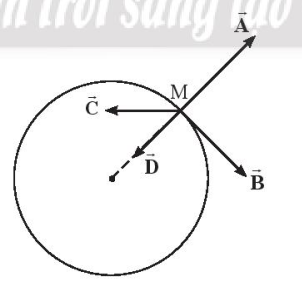
\includegraphics[width=0.3\linewidth]{../figs/0008-1VN10-2023-PH-TP0008-1}
		\captionof{figure}{}
		\label{fig:0008-1}
	\end{center}
\begin{mcq}(2)
	\item $\vec A$ là vectơ vận tốc, $\vec B$ là vectơ gia tốc.
	\item $\vec B$ là vectơ vận tốc, $\vec A$ là vectơ gia tốc.
	\item $\vec B$ là vectơ vận tốc, $\vec D$ là vectơ gia tốc.
	\item $\vec C$ là vectơ vận tốc, $\vec D$ là vectơ gia tốc.
\end{mcq}
}
\hideall{
\textbf{Đáp án C.}
}

\item \mkstar{2}\\
{Để chuyển đổi đơn vị số đo một góc từ $\si{\radian}$ (radian) sang độ và ngược lại, từ độ sang rad, hệ thức nào sau đây \textbf{không} đúng?
	\begin{mcq}(2)
		\item $\xsi{\alpha}{\degree}=\dfrac{\SI{180}{\degree}}{\pi}\cdot\xsi{\alpha}{\radian}$.
		\item $\SI{60}{\degree}=\dfrac{\SI{180}{\degree}}{\pi}\cdot\xsi{\dfrac{\pi}{3}}{\radian}$.
		\item $\SI{45}{\degree}=\dfrac{\SI{180}{\degree}}{\pi}\cdot\xsi{\dfrac{\pi}{8}}{\radian}$.
		\item $\xsi{\dfrac{\pi}{2}}{\radian}=\dfrac{\SI{180}{\degree}}{\pi}\cdot\dfrac{\pi}{2}$.
	\end{mcq}
	
}
\hideall{
	\textbf{Đáp án C.}\\
	$$\SI{45}{\degree}=\dfrac{\SI{180}{\degree}}{\pi}\cdot\xsi{\dfrac{\pi}{4}}{\radian}.$$
	}

	\item \mkstar{2}
	
	
	{Chọn câu trả lời đúng. Một quạt máy quay được 180 vòng trong thời gian $\SI{30}{s}$, cánh quạt dài $\SI{0,4}{m}$. Tốc độ dài của một điểm ở đầu cánh quạt là 
		\begin{mcq}(4)
			\item $\xsi{\dfrac{\pi}{3}}{m/s}$.
			\item 2,4$\xsi{\pi}{m/s}.$
			\item 4,8$\xsi{\pi}{m/s}.$
			\item Một giá trị khác.
		\end{mcq}
	}
	
	\hideall
	{	
		\textbf{Đáp án: C.}
		
		Tần số:
		
		$$f = \dfrac{180}{30} = \SI{6}{Hz}.$$
		
		Tần số góc:
		
		$$\omega = 2\pi f = \xsi{12\pi}{rad/s}.$$
		
		Vận tốc dài của một điểm ở đầu cánh quạt:
		
		$$v = \omega r = \text{4,8}\xsi{\pi}{m/s}.$$
	}
	\item \mkstar{2}
	
	
	{ Chọn câu trả lời đúng. Một chất điểm chuyển động trên một đường tròn bán kính $R = \SI{15}{m}$, với tốc độ dài $\SI{54}{km/h}$. Gia tốc hướng tâm của chất điểm là 
		\begin{mcq}(4)
			\item $\SI{1}{m/s^2}.$
			\item $\SI{15}{m/s^2}.$
			\item $\SI{225}{m/s^2}.$
			\item Một giá trị khác.
		\end{mcq}
	}
	
	\hideall
	{	
		\textbf{Đáp án: B.}
		
		Đổi $\SI{54}{km/h} = \SI{15}{m/s}.$
		
		Áp dụng công thức tính gia tốc hướng tâm ta có:
		
		$$a = \dfrac{v^2}{r} = \SI{15}{m/s}^2.$$
	}

	
	
	\item \mkstar{2}
	
	
	{Mặt Trăng chuyển động tròn đều quanh Trái Đất trên quỹ đạo có bán kính là 3,84 $\cdot \xsi{10^5}{km}$ và chu kì quay là 27,32 ngày. Tính gia tốc của Mặt Trăng.
		\begin{mcq}(2)
			\item $a = \text{2,7} \xsi{\cdot 10^{-3}}{m/s^2}.$ 
			\item $a = \text{2,7} \xsi{\cdot 10^{-6}}{m/s^2}.$
			\item $a = \xsi{27 \cdot 10^{-3}}{m/s^2}.$ 
			\item $a = \text{7,2} \xsi{\cdot 10^{-3}}{m/s^2}.$
		\end{mcq}
	}
	
	\hideall
	{	
		\textbf{Đáp án: A.}
		
		$$T = \text{27,32}\ \text{ngày} = \SI{2360448}{s}.$$
		
		Tốc độ góc:
		
		$$\omega = \dfrac{2\pi}{T} = \text{2,66} \xsi{\cdot 10^{-6}}{rad/s}.$$
		
		Gia tốc:
		
		$$a = r \omega^2 = \text{2,72} \xsi{\cdot 10^{-3}}{m/s}^2.$$
	}
	
	\item \mkstar{2}
	
	
	{Một chiếc xe đạp chuyển động đều trên một đường tròn bán kính $\SI{100}{m}$. Xe chạy một vòng hết 2 phút. Xác định gia tốc hướng tâm của xe.
		\begin{mcq}(4)
			\item $a = \SI{0,27}{m/s^2}.$
			\item $a = \SI{1,097}{m/s^2}.$
			\item $a = \SI{2,7}{m/s^2}.$
			\item $a = \SI{0,0523}{m/s^2}.$
		\end{mcq}
	}
	
	\hideall
	{	
		\textbf{Đáp án: A.}
		
		Đổi $T = 2\ \text{phút} = \SI{120}{s}.$
		
		Tốc độ góc:
		
		$$\omega = \dfrac{2\pi}{T} = \xsi{\dfrac{\pi}{60}}{rad/s}.$$
		
		Gia tốc hướng tâm:
		
		$$a_\text{ht} = \omega^2 R = \SI{0,274}{m/s}^2.$$
	}
	
	\item \mkstar{2}\\
	{Một vật nhỏ khối lượng $\SI{150}{\gram}$ chuyển động tròn đều trên quỹ đạo có bán kính $\SI{1.5}{\meter}$ với tốc độ $\SI{2}{\meter/\second}$. Độ lớn lực hướng tâm gây ra chuyển động tròn của vật là
		\begin{mcq}(4)
			\item $\SI{0.13}{\newton}$.
			\item $\SI{0.2}{\newton}$.
			\item $\SI{1.0}{\newton}$.
			\item $\SI{0.4}{\newton}$.
		\end{mcq}
	
}
\hideall{
\textbf{Đáp án D.}\\
Độ lớn lực hướng tâm gây ra chuyển động tròn của vật:
$$F_\text{ht}=m\dfrac{v^2}{R}=\left(\SI{0.15}{\kilogram}\right)\cdot\dfrac{\left(\SI{2}{\meter/\second}\right)^2}{\SI{1.5}{\meter}}=\SI{0.4}{\newton}.$$
}
	
	\item \mkstar{3}\\
	{Một vệ tinh khối lượng $\SI{100}{\kilogram}$, được phóng lên quỹ đạo quanh Trái Đất ở độ cao mà tại đó nó có trọng lượng $\SI{920}{\newton}$. Chu kì của vệ tinh là $\SI{5.3E3}{\second}$. Biết bán kính Trái Đất là $\SI{6400}{\kilo\meter}$. Khoảng cách từ bề mặt Trái Đất đến vệ tinh bằng
	\begin{mcq}(4)
		\item $\SI{135}{\kilo\meter}$.
		\item $\SI{146}{\kilo\meter}$.
		\item $\SI{185}{\kilo\meter}$.
		\item $\SI{153}{\kilo\meter}$.
	\end{mcq}
}
\hideall{
\textbf{Đáp án D.}\\
Lực hấp dẫn do Trái Đất tác dụng lên vệ tinh đóng vai trò là lực hướng tâm:
$$F_\text{ht}=P=m\omega^2\left(R+h\right)$$
$$\Leftrightarrow P=m\left(\dfrac{2\pi}{T}\right)^2\left(R+h\right)$$
$$\Rightarrow h=\dfrac{P}{m\cdot\left(\dfrac{2\pi}{T}\right)^2}-R=\dfrac{\SI{920}{\newton}}{\left(\SI{100}{\kilogram}\right)\cdot\left(\dfrac{2\pi}{\SI{5.3E3}{\second}}\right)^2}-\SI{6400E3}{\meter}\approx\SI{146E3}{\meter}=\SI{146}{\kilo\meter}.$$
}
	
	\item \mkstar{3}
	
	
	{Vòng xiếc là một vành tròn bán kính $R = \SI{8}{m}$, nằm trong mặt phẳng thẳng đứng. Một người đi xe đạp trên vòng xiếc này, khối lượng cả xe và người là $\SI{80}{kg}$. Lấy $g = \SI{9,8}{m/s^2}$. Lực ép của xe lên vòng xiếc tại điểm cao nhất với tốc độ tại điểm này là $v = \SI{10}{m/s}$ bằng
		\begin{mcq}(4)
			\item $\SI{164}{N}.$
			\item $\SI{186}{N}.$
			\item $\SI{254}{N}.$
			\item $\SI{216}{N}.$
		\end{mcq}
	}
	
	\hideall
	{	
		\textbf{Đáp án: D.}
		
		\begin{center}
			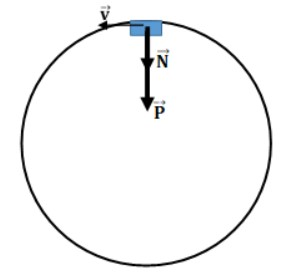
\includegraphics[scale=0.6]{../figs/VN10-2022-PH-TP0005-1.jpg}
		\end{center}
		
		Tại điểm cao nhất của vòng xiếc có các lực tác dụng lên xe là trọng lực $\vec P$ và phản lực $\vec N$ của vòng xiếc.
		
		Ta có:
		
		$$P + N = F_\text{ht} = m \dfrac{v^2}{R} \Rightarrow N = m \dfrac{v^2}{R} - P.$$
		
		Gọi $\vec N'$ là lực ép của người đi xe lên vòng xiếc, ta có:
		
		$$N' = N = \dfrac{mv^2}{R} - mg = \SI{216}{N}.$$
	}
	\item \mkstar{3}
	
	
	{Xe có khối lượng 1 tấn đi qua cầu vồng. Cầu có bán kính cong là $\SI{50}{m}$. Giả sử xe chuyển động đều với tốc độ $\SI{10}{m/s}$. Lấy $g = \SI{9,8}{m/s}^2$. Tại đỉnh cầu, lực nén của xe lên cầu bằng
		\begin{mcq}(4)
			\item $\SI{7200}{N}.$
			\item $\SI{5500}{N}.$
			\item $\SI{7800}{N}.$
			\item $\SI{6500}{N}.$
		\end{mcq}
	}
	
	\hideall
	{	
		\textbf{Đáp án: C.}
		
		\begin{center}
			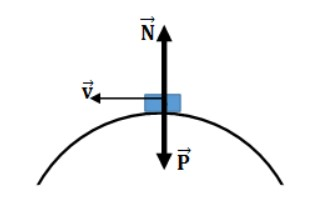
\includegraphics[scale=0.6]{../figs/VN10-2022-PH-TP0005-3.jpg}
		\end{center}
		
		Hợp lực của trọng lực $\vec P$ và lực nâng $\vec N$ của mặt cầu tác dụng lên xe đóng vai trò là lực hướng tâm.
		
		Tại điểm cao nhất áp lực ô tô lên mặt đường là
		
		$$ N = P - F_\text{ht} = mg - \dfrac{mv^2}{R} = \SI{7800}{N}.$$
	}
	
	
	\item \mkstar{3}
	
	
	{Cho một bàn tròn có bán kính $\SI{100}{\centi\meter}$. Lấy một vật có khối lượng $\SI{100}{\gram}$ đặt lên mép bàn tròn. Khi bàn tròn quay quanh một trục thẳng qua tâm bàn thì thấy vật quay đều theo bàn với tốc độ $v=\SI{10}{\meter/\second}$. Xác định hệ số ma nghỉ giữa vật và bàn tròn để vật không trượt
		\begin{mcq}(4)
			\item 10.
			\item 6.
			\item 4.
			\item 7.
		\end{mcq}
	}
	
	\hideall
	{	\textbf{Đáp án: A.}
		
	Trong quá trình bàn quay lực ma sát nghỉ giữa vật và bàn đóng vai trò là lực hướng tâm làm cho vật chuyển động tròn đều:
\begin{eqnarray*}
	&&F_\text{ht}=F_\text{msn}\le F_\text{msn max}\\
	&\Leftrightarrow& \dfrac{mv^2}{R}\le \mu mg\\
	&\Rightarrow& \mu \ge \dfrac{v^2}{gR}=10.
\end{eqnarray*}

	}
	
	
	\item \mkstar{3}\\
	{Một vệ tinh nhân tạo chuyển động tròn đều quanh Trái Đất ở độ cao bằng bán kính $R$ của Trái Đất. Lấy gia tốc rơi tự do tại mặt đất là $g=\SI{10}{\meter/\second^2}$ và bán kính của Trái Đất bằng $R=\SI{6400}{\kilo\meter}$. Chu kì quay quanh Trái Đất của vệ tinh là
		\begin{mcq}(4)
			\item 2 giờ 48 phút.
			\item  1 giờ 59 phút.
			\item 3 giờ 57 phút.
			\item  1 giờ 24 phút.
		\end{mcq}
	
}
\hideall{
\textbf{Đáp án B.}\\
$$g=\dfrac{v^2}{R+R}\Rightarrow v=\sqrt{2Rg}$$
$$\Rightarrow T=\dfrac{2\pi\cdot2R}{v}=\dfrac{4\pi R}{\sqrt{2Rg}}=\dfrac{4\pi\sqrt{R}}{\sqrt{2g}}=\dfrac{4\pi\cdot\sqrt{\SI{6400E3}{\meter}}}{\sqrt{2\cdot\left(\SI{10}{\meter/\second^2}\right)}}=\SI{7108}{\second}=1\ \text{giờ}\ 59\ \text{phút}.$$
}

\item \mkstar{3}\\
{Một đồng hồ treo tường có kim giờ dài $\SI{5}{\centi\meter}$, kim phút dài $\SI{6}{\centi\meter}$ đang chạy đúng. Xem đầu mút các kim chuyển động tròn đều. Tỉ số giữa gia tốc hướng tâm của đầu kim phút với đầu kim giờ gần giá trị nào nhất sau đây?
\begin{mcq}(4)
	\item 173.
	\item 181.
	\item 691.
	\item 120.
\end{mcq}
}
\hideall{
\textbf{Đáp án A.}\\
Chu kì quay của kim giờ và kim phút:
$$T_h=\SI{12}{\hour};\quad T_m=\SI{1}{\hour}$$
Tỉ số gia tốc hướng tâm của đầu kim phút và đầu kim giờ:
$$\dfrac{a_m}{a_h}=\dfrac{\omega^2_mR_m}{a^2_hR_h}=\left(\dfrac{T_h}{T_m}\right)^2\cdot\dfrac{R_m}{R_h}=12^2\cdot\dfrac{6}{5}=172,8.$$
}

\item \mkstar{4}\\
{Dùng một dây nhẹ, không dãn để quay một vật có khối lượng $m=\SI{500}{\gram}$ chuyển động tròn đều trong một mặt phẳng nằm ngang. Biết $g =\SI{10}{\meter/\second^2}$ và dây hợp với phương thẳng đứng một góc $\SI{60}{\degree}$. Lực căng dây có độ lớn là
\begin{mcq}(4)
	\item $\SI{5}{\newton}$.
	\item $\xsi{5\sqrt{3}}{\newton}$.
	\item $\SI{10}{\newton}.$
	\item $\xsi{\dfrac{10\sqrt{3}}{3}}{\newton}$.
\end{mcq}
}
\hideall{
\textbf{Đáp án C.}\\
Hợp lực của trọng lực $\vec P$ và lực căng dây $\vec T$ đóng vai trò là lực hướng tâm giữ cho vật nặng chuyển động tròn đều
$$\vec P+\vec T=\vec F_\text{ht}$$
Lực căng dây:
$$T=\dfrac{P}{\cos\SI{60}{\degree}}=\SI{10}{\newton}.$$
}
\end{enumerate}